\chapter{Einleitung}
\label{einleitung}


%\epigraph{e.g. Zitat}{--- \textup{Sebastian Wayne}, 2018}

Wenn Menschen von künstlicher Intelligenz (KI) hören, dann denken nicht wenige an Roboter, die sich intelligent verhalten \cite[S. 1]{Geron}. Mit Robotern wird schnell auch die Automatisierung von Abläufen in Verbindung gebracht. Aus Automatisierung folgen Effizienz und Produktivitätssteigerungen. In Folge dessen ist es nicht verwunderlich, dass mehr als die Hälfte der in einer Studie befragten Entscheider künstliche Intelligenz für das eigene Unternehmen als ein Thema mit großer oder sehr großer Relevanz bewerten, wie eine Statista-Studie (vgl. Abbildung \ref{Abbildung:statista}) zeigt. 

\begin{figure}[h]
\centering
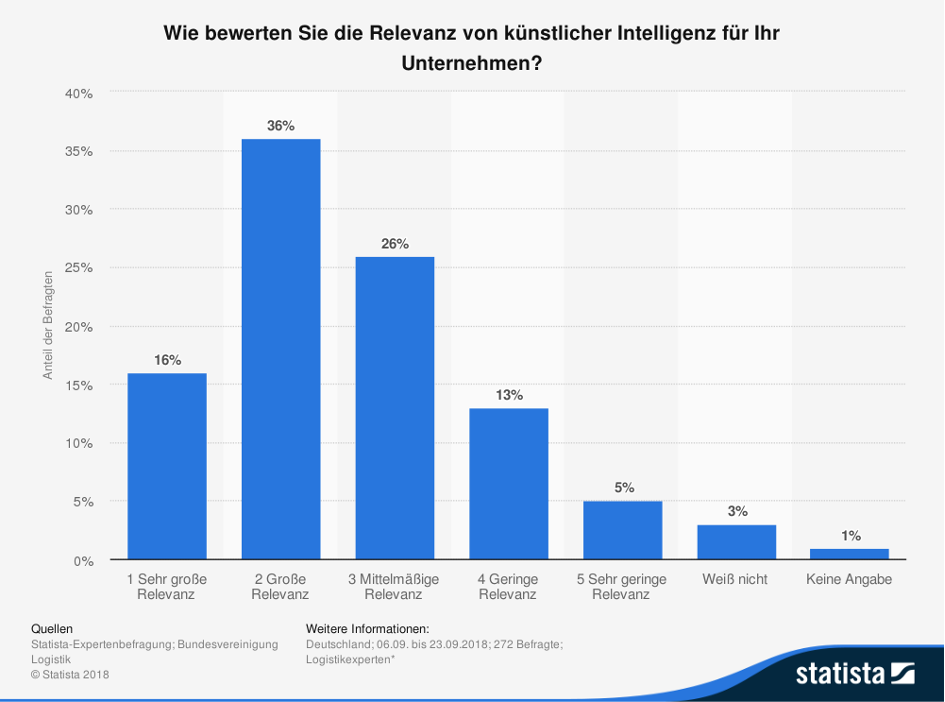
\includegraphics[scale=0.95]{content/pics/Picture_1.png}
\caption{Bewertung der Relevanz von künstlicher Intelligenz. Quelle: Statista \cite{Statista}}
\label{Abbildung:statista}
\end{figure}

Da in der Statista-Studie Experten der Logistikbranche befragt wurden, haben möglicherweise viele Teilnehmer tatsächlich an die Optimierung der Betriebskosten durch den Einsatz von Robotern in den Verteilzentren oder an selbstfahrende Lieferwagen gedacht. Der Gedanke liegt allerdings nahe, dass auch an Ansätze aus dem Gebiet des maschinellen Lernens (Engl.: Machine-Learning, Abk.: ML) gedacht wurde, um bestimmte organisatorische oder prozessuale Abläufe zu unterstützen. Das könnten Abläufe in der Verwaltung, im Vertrieb oder im Marketing, oder auch in der IT-Governance sein.

\section{Forschungsfrage- und Methode}

Der Fokus dieser Arbeit liegt speziell auf dem Application-Portfolio-Management (APM) als Teilbereich der IT-Governance. 

IT-Governance soll stets sicherstellen, dass mit Hilfe von IT die Unternehmensziele erreicht werden. Insbesondere der verantwortungsvolle Einsatz von Ressourcen ist dabei wichtig \cite{rueter}. Zur Erreichung der Unternehmensziele kommen in Unternehmen Applikationen zum Einsatz. Daraus ergeben sich Applikationslandschaften. Mit der Reduzierung der Komplexität solcher Landschaften oder auch Portfolios befasst sich das APM \cite{schoder}. 

Es sollen in dieser Arbeit Maßnahmen zur Erreichung bestimmter Ziele aus dem Bereich des APM formuliert werden. Dabei soll ganz konkret evaluiert werden, welche Maßnahmen zur Zielerreichung geeignet sind und welche nicht. Insbesondere die Chancen, die durch den Einsatz bestimmter Machine-Learning-Verfahren entstehen, sind im Kontext des APM zu bewerten. Die zu beantwortende Frage lautet demnach: 

{\bf Können ausgewählte Machine-Learning-Verfahren sinnvoll im Kontext des APM eingesetzt werden und einen echten Mehrwert erbringen?}

Die Forschungsfrage wird durch eigene Untersuchungen und Tests beantwortet. Da in einem Unternehmenskontext gearbeitet wird, sollen verschiedene Verfahren auf reale Problemstellungen angewendet werden. Es wird explorativ vorgegangen. Ansätze werden in Python implementiert und damit erprobt, im Anschluss erfolgt eine Bewertung der Ergebnisse. Für die Bewertung verwendet werden objektive Kriterien, die in Abschnitt 3.5 beschrieben werden. Der Forschungsansatz orientiert sich an der Methode Action Research. Dabei wird den Forschenden nahe gelegt, Ansätze aus der Theorie in Zusammenarbeit mit Praktikern auf reale Probleme anzuwenden \cite{Avison}. 


\section{Ziele und Aufbau der Arbeit}

Das eigentliche Ziel der Arbeit ist eine Untersuchung von ML-Verfahren, die für die Unterstützung des APM in Frage kommen. Dabei wird zunächst beschrieben, wie die jeweiligen Verfahren potenziell einen Mehrwert für das APM erbringen können. Die Verfahren werden dann evaluiert und miteinander verglichen, was letztendlich zu einer Bewertung von verschiedenen Verfahren führt. Es sollen damit Lösungsansätze für den Umgang mit Applikationsportfolios aufgezeigt werden. Wie später gezeigt wird, spielen bestimmte Text-Dokumente eine wesentliche Rolle im APM. Daher kommen insbesondere Verfahren zur Auswertung von Text-Dokumenten in Frage. 

Nach der Einführung folgt ein Grundlagenkapitel, das die notwendigen Begriffe definiert und das Thema der Arbeit detailliert beschreibt. Es wird auf wesentliche, aktuelle Fortschritte aus der Forschung eingegangen, wobei zu berücksichtigen ist, dass sich das ML-Gebiet in sehr hoher Geschwindigkeit weiterentwickelt und aus diversen Richtungen beeinflusst wird \cite[S. 146]{Gupta}. Es soll außerdem beschrieben werden, mit welchen Fragestellungen sich das APM beschäftigt. Eine Abgrenzung zur IT-Governance wird dabei vorgenommen. Im Anschluss an den Theorieteil wird das Umfeld beschrieben, in dem die Evaluation stattfindet. Es wird außerdem beschrieben, auf welche Art und Weise eine Evaluation von ML-Verfahren im gegebenen Umfeld durchgeführt werden kann. Es werden Kriterien für die Evaluation aufgestellt. Die Ergebnisse der Evaluation werden danach beschrieben. Das Fazit beendet die Arbeit.

\section{Themeneingrenzung}

Es wird in der vorliegenden Arbeit nicht vollumfänglich die historische Entwicklung des Themenbereichs KI diskutiert. Ebenfalls nicht behandelt werden philosophische oder ethische Fragestellungen, sofern diese nicht unmittelbare Auswirkungen für das Thema IT-Governance oder das Application-Portfolio-Management haben. Es soll aber ausdrücklich betont werden, dass KI-Systeme neben möglichen positiven Auswirkungen auch das Potenzial haben, die Arbeits- und Lebensrealität von Menschen negativ zu beeinträchtigen. Für eine ausführliche Diskussion dazu wird allerdings auf die einschlägige Literatur verwiesen, z. B. auf \cite[S. 11-16]{Ertel}. Die Master-Thesis soll sich hingegen inhaltlich auf aktuelle technische und für den Anwendungsfall relevante betriebswirtschaftliche Aspekte konzentrieren. 
Aufgrund der begrenzten Bearbeitungszeit kann nur eine gewisse Auswahl an ML-Verfahren berücksichtigt werden.

%\subsection{Allgemeines zum Crawler}
